% \newpage
\section{Evaluation} \label{sec:eval}

As part of \xxx's development, we have implemented a fast RDMA-enabled \paxos 
protocol~\cite{falcon:github} for general applications. We evaluated this 
protocol with \redis~\cite{redis}, a popular key-value store. We chose \redis 
because it complies with a social-networking platform setting, where 
high-availability is important (\S\ref{sec:discuss}).

For instance, Twitter uses \mesos as its scheduler and runs \redis as its core 
key-value store. Key-value stores are also widely used in critical, financial 
applications~\cite{nosql:finance,nosql:racs14}. In our evaluation, \xxx 
transparently supported \redis without the need of modifying \redis's code. 

% Evaluation machine and workloads.
Our evaluation used three Dell R430 servers as SMR replicas. Each server has 
Linux 3.16.0, 2.6 GHz Intel Xeon CPU with 24 hyper-threading cores, 64GB 
memory, and 1TB SSD. Each machine has a Mellanox ConnectX-3 Pro Dual Port 40 
Gbps NIC. These NICs are connected using the Infiniband RDMA architecture.

To mitigate network latency of public network, benchmarks were ran 
in a Dell R320 server (the application scheduler machine), with Linux 3.16.0, 
2.2GHz Intel Xeon 12 hyper-threading cores, 32GB memory, and 160GB SSD. This 
server connects with the server machines with 1Gbps bandwidth LAN. The average 
\v{ping} latency between the benchmark machine and a server machine is 301 \us. 
A larger network latency (\eg, sending job requests from WAN) will further 
mask \xxx's overhead.

To perform a stress testing on \xxx's input consensus protocol, we chose 
\redis's own benchmark to spawn a workload with 50\% SET and 50\% GET 
operations. We chose such a significant portions of writes because SET 
operation contains more bytes than a GET.

We spawned up to 32 concurrent connections, and then we measured both response 
time and throughput. We also measured \xxx's bare consensus latency. All 
evaluation results were done with a replica group size of three. Each 
performance data point in the evaluation is taken from the mean value of 10 
repeated executions.

The rest of this section focuses on these questions:

\begin{tightenum}

\item[\S\ref{sec:overhead}:] What is \xxx's performance compared to the 
unreplicated executions? What is the consensus latency of \xxx's \paxos 
protocol?

\item[\S\ref{sec:compare}:] What is \xxx's performance compared to existing 
SMR systems?


% \item[\S\ref{sec:scalability}:] How scalable is \xxx on different replica group 
% sizes?

\end{tightenum}

\subsection{Performance Overhead} \label{sec:overhead}

Figure~\ref{fig:tput} shows \xxx's throughput and 
Figure~\ref{fig:latency} response time. We varied the number of concurrent 
benchmark connections for each server program by from one to 32 threads. 
Overall, compared to \redis's unreplicated executions, \xxx merely incurred a 
mean throughput overhead of \tputoverhead.

As the number of threads increases, \redis's unreplicated executions 
got a performance improvement. \xxx scaled almost as well as the unreplicated 
executions.

\begin{figure}[h]
\centering
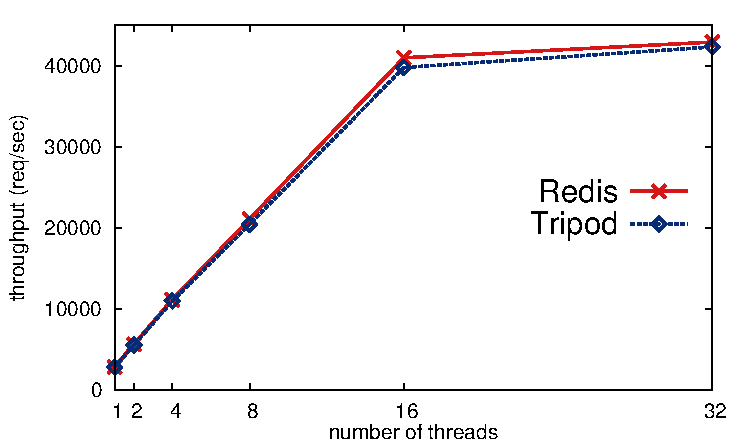
\includegraphics[width=0.47\textwidth]{figures/throughput}
% \vspace{-.10in}
\caption{\small {\em \xxx throughput compared to the unreplicated 
execution.}}
% \vspace{-.20in}
\label{fig:tput}
\end{figure}
 
\begin{figure}[h]
\centering
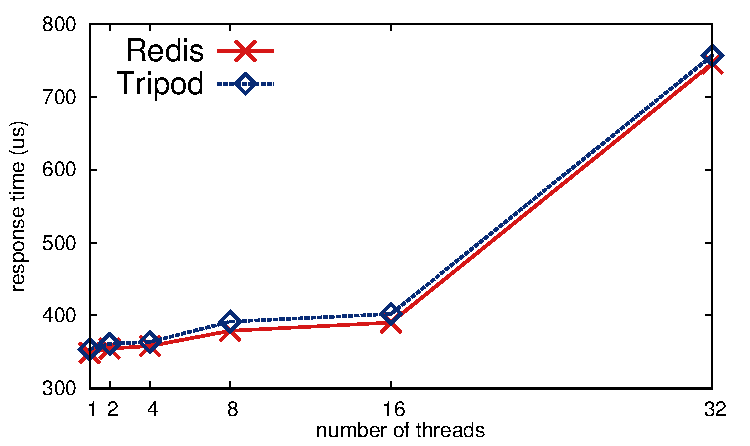
\includegraphics[width=0.47\textwidth]{figures/latency}
% \vspace{-.10in}
\caption{\small {\em \xxx response time compared to the unreplicated 
execution.}}
% \vspace{-.20in}
\label{fig:latency}
\end{figure}

To deeply understand \xxx's performance overhead, we collected the number of 
socket call events and consensus durations on the leader controller side. Given 
10K requests and 8 concurrent connections, \redis spawned 10,016 socket calls, 
each of which invoked a \paxos consensus. The average received data bytes in 
these socket calls were 42.0 (\eg, inputs from \recv). The average consensus 
latency for these calls were 9.9 \us because consensus were done by RDMA WRITEs 
across the leader and standby masters.

These results suggest that \xxx has the potential to provide a fast 
\paxos replication service to general applications with low overhead. 

\subsection{Comparison with Traditional SMR Systems} \label{sec:compare}

\begin{table}[h]
\footnotesize
\centering
% \vspace{-.2in}
\begin{tabular}{lrr}
{\bf Performance metric} & {\bf \zookeeper} & {\bf \xxx}\\
\hline\\[-2.3ex]
Throughput (requests/s) & 19,925   & 17,614 \\
Consensus latency (\us) & 511.9  & 12.5\\
\end{tabular}
% \vspace{-.1in}
\caption{{\em Comparison with \calvin's \zookeeper replication.}} 
% \vspace{-.2in}
\label{tab:compare}
\end{table}

We compared \xxx with the \calvin database system~\cite{calvin:sigmod12} 
because \calvin's input consensus uses \zookeeper~\cite{zookeeper}, one of the 
most widely used coordination service built on TCP/IP. To conduct a fair 
comparison, we ran \calvin's own transactional database server in \xxx as the 
server program, and we compared throughputs and the consensus latency with 
\calvin's consensus protocol \zookeeper.

As shown in Table~\ref{tab:compare}, \calvin's \zookeeper replication achieved 
19.9K transactions/s with a 511.9 \us consensus latency. \xxx achieved 17.6K 
transactions/s with a 12.5 \us consensus latency. The throughput in \calvin 
was 13.1\% higher than that in \xxx because \calvin puts transactions in a 
batch with a 10 \ms timeout, it then invokes \zookeeper for consensus on 
this batch. The average number of bytes in \calvin's batches is 18.8KB, and 
the average number of input bytes in each \xxx consensus (one for each \recv 
call) is 93 bytes. Batching helps \calvin achieve good throughput. \xxx 
currently has not incorporated a batching technique because its latency is 
already reasonable (\S\ref{sec:overhead}).

Notably, \xxx's consensus latency was 40.1X faster than \zookeeper's mainly due 
to \xxx's RDMA-accelerated consensus protocol, although we ran \calvin's 
\zookeeper consensus on IPoIB. A prior SMR evaluation~\cite{dare:hpdc15} also 
reports a similar 320 \us consensus latency in \zookeeper. Two other recent SMR 
systems Crane~\cite{crane:sosp15} and Rex~\cite{rex:eurosys14} may incur 
similar consensus latency as \zookeeper's because all their consensus protocols 
are based on TCP/IP.

This comparison shows that \xxx's \paxos protocol can be leveraged to speedup 
the SMR services in existing cluster management systems (\eg, \mesos currently 
uses \zookeeper).



% Results: tput, latency.

% \subsection{Performance Overhead of \xxx's \paxos protocol} \label{sec:overhead}



% \subsection{Response Times in Critical Application Workloads} 
% \label{sec:workload}
% 
% TBD.

